% Copyright 2005 by Till Tantau <tantau@cs.tu-berlin.de>.
%
% This program can be redistributed and/or modified under the terms
% of the LaTeX Project Public License Distributed from CTAN
% archives in directory macros/latex/base/lppl.txt.


\section{Watching Trees Grow}

\label{section-trees}


\subsection{Introduction to the  Child Operation}

\emph{Trees} are a common way of visualizing hierarchical
structures. A simple tree looks like this:
\begin{codeexample}[]
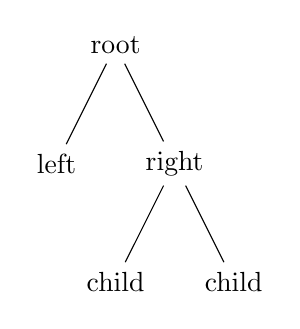
\begin{tikzpicture}
  \node {root}
    child {node {left}}
    child {node {right}
      child {node {child}}
      child {node {child}}
    };
\end{tikzpicture}
\end{codeexample}

Admittedly, in reality trees are more likely to grow \emph{upward} and
not downward as above. This is easy enough to specify in \tikzname:

\begin{codeexample}[]
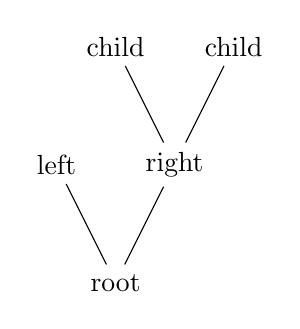
\begin{tikzpicture}
  \node {root} [grow'=up]
    child {node {left}}
    child {node {right}
      child {node {child}}
      child {node {child}}
    };
\end{tikzpicture}
\end{codeexample}

(You can tell whether the author of a paper is a mathematician or a
computer scientist by looking at the direction their trees grow. A
computer scientist's trees will grow downward while a mathematician's
tree will upward. Naturally, the correct way is the mathematician's
way.)

In \tikzname, trees are specified by adding \emph{child nodes} to a
node on a path. The syntax for the child operation is the following:

\begin{pathoperation}{child}{\opt{\oarg{options}}\opt{\marg{child path}}}
  This operation should directly follow a completed |node| operation
  or another |child| operation, although it is permissible that the
  first |child| operation is preceded by options (we will come to
  that).

  The exact effects of this operation are described in the rest of
  this present section.
\end{pathoperation}





\subsection{Where Children and Their Options Are Specified}

When a |node| operation like |node {X}| is followed by |child|,
\tikzname\ starts counting the number of child nodes that follow the
original |node {X}|. For this, it scans the input and stores away each
|child| and its arguments until it reaches a path operation that is
not a |child|. Note that this will fix the character codes or any
text inside the child arguments, which means, in essence, that you
cannot use verbatim text inside the nodes inside a |child|. Sorry. 

Once the children have been collected and counted, \tikzname\ starts
generating the nodes of the children.

Each |child| may have its own \meta{options}, which apply to ``the
whole child,'' including all of its grandchildren. Here is an
example:

\begin{codeexample}[]
\begin{tikzpicture}[thick,sibling distance=10mm on level 2]
  \coordinate
    child[red]   {child child}
    child[green] {child child[blue]};
\end{tikzpicture}
\end{codeexample}

The options of the root node have no effect on the children since
the options of a node are always ``local'' to that node. Because of
this, the edges in the following tree are black, not red.
  
\begin{codeexample}[]
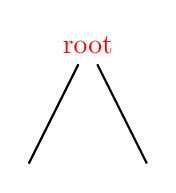
\begin{tikzpicture}[thick]
  \node [red] {root}
    child
    child;
\end{tikzpicture}
\end{codeexample}
  This raises the problem of how to set options for \emph{all}
  children. Naturally, you could always set options for the whole path
  as in |\path [red] node {root} child child;| but this is bothersome
  in some situations. Instead, it is easier to give the options
  \emph{before the first child} as follows:
\begin{codeexample}[]
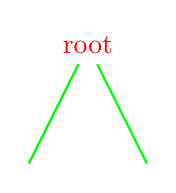
\begin{tikzpicture}[thick]
  \node [red] {root}
    [green] % option applies to all children
    child
    child;
\end{tikzpicture}
\end{codeexample}

To sum up: Options for the whole tree are given before the root
node. Options for the root node are given directly to the |node|
operation of the root. Options for all children can be given between
the root node and the first child. Options applying to a specific
child are given as options to the child.


\subsection{The Shapes and Content Child Nodes}

For each |child| of a root node, a node is generated and placed
somewhere (the placement rules will be discussed later). The shape of
the child node depends on the \meta{child path} of the child.

In the easiest case, the \meta{child path} is completely missing
(including the curly braces). An example would be
|\node {x} child child;| where both children miss their \meta{child
  path}. In this case the shape is simply a |coordinate|. Thus, the
child node has no extend and no text. 
\begin{codeexample}[]
\tikz \node {root} child child;
\end{codeexample}

Next, the \meta{child path} may \emph{start} with a |node| or a
|coordinate| specification. An example is
|\node {x} child {node {y}};| where the \meta{child path} consists
of the node specification  |node {y}|. In this case, this first node
on the path becomes the child node. As for any normal node, you can
give this child node a name, shift it around, or use options to
influence how it is rendered.
\begin{codeexample}[]
\begin{tikzpicture}
  \node[rectangle,draw] {root}
    child {node[circle,draw] (left node) {left}}
    child {node[ellipse,draw] (right node) {right}};
  \draw[dashed,->] (left node) -- (right node);
\end{tikzpicture}
\end{codeexample}

A third case occurs when the \meta{child path} exists, but does not
start with a |node| or |coordinate| as in
|child {child};|, where the \meta{child path} start with |child|
itself. In this case, a node of shape |coordinate| is automatically
added at the beginning of the path. 

\subsection{The Placement of Child Nodes}

\subsection{The Edge From the Parent Node}





%%% Local Variables: 
%%% mode: latex
%%% TeX-master: "pgfmanual"
%%% End: 
